\documentclass[UTF8,a4paper]{ctexart}

\usepackage{geometry}
\usepackage{graphicx}
\usepackage{float}
\usepackage{amsmath}
\usepackage{booktabs}
\usepackage{array}
\usepackage{tabularx}
\usepackage{ragged2e}
\usepackage{listings}
\usepackage{algorithm}
\usepackage{algpseudocode}
\usepackage{xcolor}
\usepackage{enumitem}
\usepackage{titlesec}
\usepackage{hyperref}

\geometry{left=2.35cm,right=2.35cm,top=2.35cm,bottom=2.35cm}
\hypersetup{colorlinks=true,linkcolor=black,urlcolor=blue}

\linespread{0.94}
\setlength{\parskip}{0pt}
\setlength{\abovedisplayskip}{4pt plus 1pt minus 1pt}
\setlength{\belowdisplayskip}{4pt plus 1pt minus 1pt}
\setlength{\abovedisplayshortskip}{3pt plus 1pt minus 1pt}
\setlength{\belowdisplayshortskip}{3pt plus 1pt minus 1pt}
\setlength{\textfloatsep}{6pt plus 1pt minus 2pt}
\setlength{\intextsep}{6pt plus 1pt minus 2pt}
\setlength{\floatsep}{5pt plus 1pt minus 1pt}
\setlength{\abovecaptionskip}{3pt}
\setlength{\belowcaptionskip}{0pt}
\setlength{\tabcolsep}{5pt}
\renewcommand{\arraystretch}{1.08}
\newcolumntype{Y}{>{\RaggedRight\arraybackslash}X}
\newcolumntype{L}[1]{>{\RaggedRight\arraybackslash}p{#1}}
\newcolumntype{R}[1]{>{\raggedleft\arraybackslash}p{#1}}
\newcolumntype{C}[1]{>{\centering\arraybackslash}p{#1}}

\setlist{nosep,leftmargin=2em,itemsep=0pt,parsep=0pt,topsep=2pt}
\titlespacing*{\section}{0pt}{0.9ex plus 0.2ex minus 0.1ex}{0.6ex plus 0.1ex}
\titlespacing*{\subsection}{0pt}{0.8ex plus 0.2ex minus 0.1ex}{0.45ex plus 0.1ex}
\titlespacing*{\subsubsection}{0pt}{0.7ex plus 0.2ex minus 0.1ex}{0.35ex plus 0.1ex}

\lstset{
  basicstyle=\small\ttfamily,
  numbers=left,
  numberstyle=\footnotesize\color{black!45},
  frame=lines,
  framerule=0.45pt,
  rulecolor=\color{black},
  breaklines=true,
  breakatwhitespace=false,
  columns=fullflexible,
  keepspaces=true,
  showstringspaces=false,
  lineskip=1pt,
  numbersep=7pt,
  xleftmargin=1.6em,
  xrightmargin=0.2em,
  aboveskip=0.65em,
  belowskip=0.65em,
  keywordstyle=\color{blue!70!black},
  commentstyle=\color{green!35!black},
  stringstyle=\color{red!55!black}
}
\floatstyle{plain}
\restylefloat{algorithm}
\floatname{algorithm}{代码}

\newcommand{\reporttitle}{并行程序设计 Lab2}

\newcommand{\coreporttitle}{矩阵 SVD 分解 SIMD 编程实验报告}
\newcommand{\reportauthor}{姓名：崔迪 \quad 学号：2412439 }

\begin{document}
\pagenumbering{gobble}
\begin{titlepage}
  \centering
  \vspace*{1.1cm}

  
\includegraphics[width=0.9\textwidth]{NKU.png}

  \vspace{2.4cm}
  {\LARGE\bfseries \reporttitle\par}
  \vspace{0.8em}
  {\Large \coreporttitle\par}

  % \vfill
  \vspace{5cm}
  {\large \reportauthor\par}

  \vspace{5cm}
  {\large \today\par}

  \vspace*{1.1cm}
\end{titlepage}
\begingroup
\normalsize
\linespread{1.18}\selectfont
\setlength{\parskip}{2pt}
\tableofcontents
\endgroup
\clearpage
\pagenumbering{arabic}
\setcounter{page}{1}

\phantomsection
\addcontentsline{toc}{section}{摘要}
\section*{摘要}

本文围绕矩阵奇异值分解（SVD）中的 Golub-Kahan 迭代和 Householder 上二对角化过程，完成了基于 AArch64 NEON intrinsic 的 SIMD 优化实验。实现部分主要包括对 GKH 简单矩阵旋转中的左行旋转进行向量化，以及对 Householder 阶段的内积、平方和和 AXPY 行更新进行 SIMD 改写，并保留尾部标量循环以处理非向量宽度整数倍的矩阵规模。实验在固定随机种子和多组矩阵规模下比较串行版本与 SIMD 版本的正确性和性能，并进一步结合不同编译优化选项、不同 SIMD 展开粒度、\texttt{perf} profiling、编译器自动向量化、ARM 与 x86 平台对比以及分块 Householder 原型进行分析。结果表明，SIMD 优化在随机 \(1000\times1000\) 样例上取得稳定加速，主配置 \texttt{-O2} 下总体加速比为 \(1.2342\times\)，收益主要来自连续访存的 Householder 相关循环；剩余瓶颈主要集中在 GKH 迭代中按列跨步访问的右旋转操作。

项目代码链接：\url{https://github.com/changluei/Parallel-Programming-Experiment}

\section{实验背景与目标}

\subsection{SVD 分解问题简介}
本文选择矩阵 SVD 算子作为实验对象，原因是该算法既包含大量规则的向量、矩阵运算，又包含较复杂的迭代与数值稳定性要求，适合观察 SIMD 对完整科学计算程序的实际影响。

奇异值分解（Singular Value Decomposition, SVD）将矩阵表示为两个正交矩阵和一个对角矩阵的乘积。对于 \(m\times n\) 实矩阵 \(A\)，其基本形式为：
\[
  A = U \Sigma V^T
\]
其中 \(U\) 和 \(V\) 分别为左、右奇异向量矩阵，\(\Sigma\) 的对角线元素为奇异值。SVD 常用于数据降维、特征提取、图像压缩、推荐系统和数值线性代数中的低秩近似等场景。由于这些应用往往需要处理较大规模矩阵，核心循环中的内积、平方和、线性组合和矩阵行列更新会成为主要计算开销，因此有必要利用 NEON、SSE/AVX 等 SIMD 指令提升单核数据级并行能力。

\subsection{Golub-Kahan 算法与实验框架}
本节概述实验框架采用的 Golub-Kahan 算法流程，重点说明本次 SIMD 优化主要涉及的两个阶段：
\begin{enumerate}
  \item GKH 迭代中的简单矩阵旋转操作；
  \item Householder 变换中的上二对角化计算。
\end{enumerate}

\subsection{实验目标}
结合实验指导书和课堂 PPT 的要求，本文的实验目标分为基础目标和进阶目标两部分。

\textbf{基础目标。} 基础部分要求在 ARM 平台上完成 SVD 框架中关键 TODO 的 SIMD 并行化，并给出正确性和性能分析：
\begin{enumerate}
  \item 实现 GKH 简单矩阵旋转中的 SIMD 加速；
  \item 实现 Householder 上二对角化过程中的 SIMD 加速；
  \item 正确处理矩阵规模不是 SIMD 向量宽度整数倍的情况，通过尾部标量循环保证结果正确；
  \item 对比串行版本与 SIMD 版本在不同测试样例、不同编译优化等级下的运行时间，并结合重构误差和正交性误差验证优化前后 SVD 结果一致；
  \item 使用 \texttt{perf} 等工具进行 profiling，结合热点函数、指令数、cycles、IPC 和 cache 行为解释程序为什么加速或为什么加速受限。
\end{enumerate}

\textbf{进阶目标。} 进阶部分希望进一步分析 SIMD 优化策略与平台、编译器和算法结构之间的关系。本文选择完成以下方向：
\begin{enumerate}
  \item 比较手工编写的 NEON SIMD 版本、编译器自动向量化版本和禁用自动向量化的标量基线，分析手写 intrinsic 与编译器优化各自贡献的性能收益；
  \item 比较 ARM NEON 与 x86 AVX 平台内加速比，避免只用绝对时间判断平台优劣，而是结合向量宽度、数据布局、访存局部性和热点阶段解释性能差异；
  \item 测试不同 SIMD 展开粒度，包括二路、四路和八路展开，分析展开因子对循环控制开销、寄存器压力和实际吞吐率的影响；
  \item 探索分块 Householder 变换等其他算法优化策略，观察其对上二对角化阶段和完整 SVD 程序总时间的不同影响。
\end{enumerate}

\section{实验环境}

\subsection{硬件环境}
本次实验除了 x86 与 ARM 平台对比部分，其余均使用 OpenEuler 服务器集群进行实验。服务器平台为 AArch64 架构，CPU 为 HiSilicon Kunpeng-920，共 8 个在线 CPU 核心。

\subsection{软件环境}
服务器端软件环境如表 \ref{tab:software} 所示。正式性能测试通过课程框架提供的 \texttt{test.sh} 脚本提交并运行；补充 profiling 和自动向量化分析则在登录节点上直接运行。

\begin{table}[H]
  \centering
  \resizebox{\textwidth}{!}{
  \begin{tabular}{p{0.22\textwidth}p{0.70\textwidth}}
    \toprule
    项目 & 版本或参数 \\
    \midrule
    操作系统与平台 & OpenEuler 服务器集群，AArch64 Linux 环境 \\
    编译器 & GCC/G++ 10.3.1 \\
    编程语言标准 & C++17 \\
    构建与运行方式 & 正式测试使用课程框架 \texttt{test.sh} 脚本 \\
    主要编译参数 & \texttt{-O0}、\texttt{-O1}、\texttt{-O2}；语言标准参数为 \texttt{-std=c++17} \\
    Profiling 工具 & Linux \texttt{perf record}、\texttt{perf report}、\texttt{perf stat} \\
    测试随机种子 & \texttt{2412439} \\
    \bottomrule
  \end{tabular}}
  \caption{实验软件环境}
  \label{tab:software}
\end{table}

\section{基础要求}

\subsection{基础要求概述}
根据实验指导书，SVD 选题的基础要求主要包括：
\begin{enumerate}
  \item 实现 \texttt{gkh.cpp} 中矩阵旋转相关 TODO 的 SIMD 加速；
  \item 实现 \texttt{bidiagonalization.cpp} 中 Householder 上二对角化相关循环的 SIMD 加速；
  \item 注意矩阵规模不一定是 SIMD 寄存器宽度的整数倍，需要正确处理剩余元素；
  \item 测试串行算法和 SIMD 算法在不同矩阵规模下的性能；
  \item 对 SIMD 是否加速以及原因进行分析；
  \item 结合测试结果进行 profiling，并对热点与瓶颈做简要分析；
  \item 测试不同并行度或不同 SIMD 宽度实现对性能的影响；
  \item 比较不同编译优化选项（无优化、\texttt{-O1}、\texttt{-O2}）对性能的影响。
\end{enumerate}

\subsection{代码改动对比}
 本次 SIMD 相关改动主要集中在两个文件中，如表 \ref{tab:code-diff} 所示。

\begin{table}[H]
  \centering
  \normalsize
  \renewcommand{\arraystretch}{1.24}
  \begin{tabularx}{\textwidth}{L{2.8cm}Y Y L{2.8cm}}
    \toprule
    \textbf{模块} & \textbf{原始实现} & \textbf{SIMD 优化实现} & \textbf{主要收益} \\
    \midrule
    GKH 左行旋转 &
    \texttt{apply\_left\_rows} 逐列标量处理两行 Givens 旋转，每次只更新一个 \texttt{double}。 &
    增加 AArch64 NEON 分支，使用 \texttt{float64x2\_t} 一次处理 2 个 \texttt{double}，并对不足一个向量宽度的尾部元素保留标量处理。 &
    减少循环指令数，提高连续行访问吞吐。 \\
    \addlinespace[0.25em]
    Householder 上二对角化 &
    Householder 变换中的内积、平方和和矩阵更新主要依赖普通双重循环，部分访问顺序与 row-major 存储不够匹配。 &
    增加 \texttt{dot\_product\_simd}、\texttt{self\_dot\_simd}、\texttt{axpy\_simd} 三个 SIMD 辅助函数，并将左右 Householder 更新改写为按行连续访问的 AXPY 形式。 &
    强化连续访存，提升大规模矩阵上二对角化阶段性能。 \\
    \bottomrule
  \end{tabularx}
  \renewcommand{\arraystretch}{1.08}
  \caption{SVD SIMD 优化代码改动对比}
  \label{tab:code-diff}
\end{table}

\subsection{简单矩阵旋转的 SIMD 加速}
本节对应 \texttt{gkh.cpp} 中的 \texttt{apply\_left\_rows} 等函数。

\subsubsection{串行计算逻辑}
原始代码逐列读取两行元素，并计算如下旋转：
\[
\begin{aligned}
  M_{r0,j}' &= cM_{r0,j} + sM_{r1,j} \\
  M_{r1,j}' &= -sM_{r0,j} + cM_{r1,j}
\end{aligned}
\]

\subsubsection{SIMD 设计思路}
\texttt{apply\_left\_rows} 的原始实现每次只处理一列。优化后先取得两行的连续内存指针 \texttt{row0} 和 \texttt{row1}，再使用 NEON 的 \texttt{float64x2\_t} 向量寄存器一次处理 2 个 \texttt{double}。核心操作是将旋转系数 $c$、$s$ 和 $-s$ 广播到向量寄存器中，对两行元素并行计算：
\[
\begin{aligned}
  \mathbf{row0}' &= c\mathbf{row0} + s\mathbf{row1} \\
  \mathbf{row1}' &= -s\mathbf{row0} + c\mathbf{row1}
\end{aligned}
\]

该实现的几个要点如下：
\begin{enumerate}
  \item 使用 AArch64 NEON 的 128 bit 寄存器，每次处理 2 个双精度浮点数；
  \item 使用 \texttt{vld1q\_f64} 和 \texttt{vst1q\_f64} 进行连续内存加载与写回；
  \item 使用 \texttt{vdupq\_n\_f64} 广播旋转系数，减少循环内重复构造；
  \item 当列数不是 2 的整数倍时，剩余 1 个元素继续使用原标量公式处理，从而保证任意矩阵规模下的正确性。
\end{enumerate}

\subsubsection{关键代码说明}
关键实现如下：

\begin{algorithm}[H]
\begin{lstlisting}[language=C++]
const float64x2_t c2 = vdupq_n_f64(c);
const float64x2_t s2 = vdupq_n_f64(s);
const float64x2_t neg_s2 = vdupq_n_f64(-s);

for (; j + 1 < cols; j += 2)
{
    const float64x2_t a = vld1q_f64(row0 + j);
    const float64x2_t b = vld1q_f64(row1 + j);

    const float64x2_t new0 = vaddq_f64(vmulq_f64(c2, a), vmulq_f64(s2, b));
    const float64x2_t new1 = vaddq_f64(vmulq_f64(neg_s2, a), vmulq_f64(c2, b));

    vst1q_f64(row0 + j, new0);
    vst1q_f64(row1 + j, new1);
}

for (; j < cols; ++j)
{
    const double a = row0[j];
    const double b = row1[j];
    row0[j] = c * a + s * b;
    row1[j] = -s * a + c * b;
}
\end{lstlisting}
\caption{gkh.cpp 中 apply\_left\_rows 的 SIMD 核心代码}
\label{alg:gkh-left-rows}
\end{algorithm}

从计算量看，每两个元素需要完成两组线性组合，包含多次乘法和加法，比较适合 SIMD。由于矩阵类按行连续存储，左乘两行时访问的是连续内存，因此 \texttt{apply\_left\_rows} 可以直接使用 \texttt{vld1q\_f64} 和 \texttt{vst1q\_f64} 做连续向量加载与写回，cache 行为也较好。相对而言，\texttt{apply\_right\_cols} 是按列访问，若矩阵使用 row-major 存储，则同一列相邻元素在内存中并不连续，不能像两行旋转那样直接用一条 NEON 连续加载指令处理。因此本次 SIMD 改写主要覆盖 \texttt{apply\_left\_rows} 以及 Householder 阶段的内积、平方和和 AXPY 行更新。

\subsection{Householder 上二对角化的 SIMD 加速}
本节对应 \texttt{bidiagonalization.cpp} 中的 Householder 变换 TODO。

\subsubsection{计算过程分析}
说明 Householder 变换：
\[
  H = I - \beta vv^T,\quad \beta = \frac{2}{v^Tv}
\]
以及从左侧作用到矩阵：
\[
  B_{new} = B_{old} - \beta v(v^TB_{old})
\]
可以拆分为向量内积、矩阵更新和累积 $U$ 的过程。

\subsubsection{可向量化循环}
优化后的 \texttt{bidiagonalization.cpp} 新增了三个可复用的 SIMD 辅助函数：
\begin{enumerate}
  \item \texttt{self\_dot\_simd}：计算 $v^Tv$ 或向量范数中的平方和；
  \item \texttt{dot\_product\_simd}：计算两个连续向量的内积；
  \item \texttt{axpy\_simd}：执行 \texttt{dst += scale * src}，用于矩阵行更新。
\end{enumerate}

这些函数的共同特点是先用 NEON 一次处理 2 个 \texttt{double}，最后用标量循环处理尾部元素。以 \texttt{axpy\_simd} 为例：

\begin{algorithm}[H]
\begin{lstlisting}[language=C++]
const float64x2_t scale2 = vdupq_n_f64(scale);
for (; i + 1 < len; i += 2)
{
    const float64x2_t dv = vld1q_f64(dst + i);
    const float64x2_t sv = vld1q_f64(src + i);
    vst1q_f64(dst + i, vaddq_f64(dv, vmulq_f64(scale2, sv)));
}

for (; i < len; ++i)
{
    dst[i] += scale * src[i];
}
\end{lstlisting}
\caption{bidiagonalization.cpp 中 axpy\_simd 的 SIMD 核心代码}
\label{alg:axpy-simd}
\end{algorithm}

在左侧 Householder 变换中，原始版本按列计算 $w[j] += v[i]B[k+i,k+j]$。由于 \texttt{Matrix} 按行连续存储，按列访问会造成较差的空间局部性。优化版本将其改写为按行 AXPY：
\[
  w \leftarrow w + v_i B_{i,:}
\]
也就是每次读取 $B$ 的一段连续行切片，并调用 \texttt{axpy\_simd} 向量化更新 $w$。随后再对每一行执行
\[
  B_{i,:} \leftarrow B_{i,:} - \beta v_i w
\]
同样可以使用 \texttt{axpy\_simd} 完成。

在累积 $U$ 时，优化版本把 $w_U = U[:,k:m]v$ 写成逐行连续内存内积，调用 \texttt{dot\_product\_simd}；随后对 $U$ 的每一行做 \texttt{axpy\_simd} 更新。右侧 Householder 变换也采用同样思路：先按行计算 $w = B_{sub}v$，再按行更新 $B$ 和 $V$。

本次实际向量化的循环包括：
\begin{enumerate}
  \item 计算 $v^Tv$ 的归约；
  \item 计算 $w = v^TB$；
  \item 更新 $B$ 的子矩阵；
  \item 计算 $w_U = Uv$；
  \item 更新 $U$ 的子矩阵。
\end{enumerate}

\subsubsection{正确性处理}
本次实现没有改变 Householder 变换的数学形式，仍然使用
\[
  H = I - \beta vv^T,\quad \beta = \frac{2}{v^Tv}
\]
并且不显式构造 $H$，而是通过内积和秩一更新直接作用到 $B$、$U$、$V$ 上。与原始版本相比，主要变化是循环顺序和单次循环处理的数据宽度。

正确性方面需要注意两点。第一，矩阵规模或子矩阵宽度不一定是 2 的整数倍，因此所有 SIMD 辅助函数都保留了尾部标量循环。第二，SIMD 归约改变了浮点加法顺序，因此结果可能与串行版本存在极小浮点误差，报告中应使用最大绝对误差或重构误差 $\|A-U\Sigma V^T\|$ 进行验证，而不应要求逐 bit 完全一致。

\begin{table}[H]
  \centering
  \begin{tabular}{cccc}
    \toprule
    矩阵规模 & 串行相对重构误差 & SIMD 相对重构误差 & 结果 \\
    \midrule
    固定值 $5\times5$ & $2.76702\times10^{-13}$ & $2.76725\times10^{-13}$ & PASS \\
    随机 $10\times8$ & $1.12970\times10^{-13}$ & $1.12775\times10^{-13}$ & PASS \\
    随机 $1000\times1000$ & $3.17504\times10^{-13}$ & $3.17875\times10^{-13}$ & PASS \\
    \bottomrule
  \end{tabular}
  \caption{代表性正确性测试结果（\texttt{-O2}）}
  \label{tab:correctness}
\end{table}

从测试结果可以看到，SIMD 版本与原始版本在所有测试用例上都满足收敛要求，且 \(\|A-U\Sigma V^T\|/\|A\|\) 维持在 \(10^{-13}\) 数量级，\(\|U^TU-I\|_F\) 和 \(\|V^TV-I\|_F\) 也保持在 \(10^{-13}\sim10^{-15}\) 范围内。这说明本次向量化虽然改变了部分浮点运算顺序，但没有破坏 SVD 分解的数值正确性。

\subsection{基础性能测试}

\subsubsection{测试方法}
测试使用框架自带的 \texttt{test.sh} 脚本完成，随机种子固定为 \texttt{2412439}，也就是我的学号，测试集包含 5 组数据：固定值 \(5\times5\)、随机 \(8\times8\)、近秩亏损 \(10\times8\)、随机 \(10\times8\) 和随机 \(1000\times1000\)。每组测试分别记录上二对角化阶段（\texttt{bidiagonalization}）和 GKH 迭代阶段（\texttt{gkh iteration}）的耗时，同时检查收敛性、重构误差、正交性误差以及奇异值排序正确性。

由于程序运行存在一定波动，因此每个版本在同一编译选项下重复运行 3 次，并将 3 次结果取平均值作为最终性能数据。基础性能分析将 \texttt{-O0/-O1/-O2} 三种编译选项下的 5 组测试统一列在同一张表中。本文后续以 \texttt{-O2} 作为主结果配置，因为它是实验中最常用的高等级编译优化选项；\texttt{-O0} 和 \texttt{-O1} 主要作为对照，用于分析编译器优化与手工 SIMD 之间的相互影响。

\subsubsection{串行版本与 SIMD 版本性能对比}

\begin{table}[H]
  \centering
  \small
  \begin{tabular}{cccccp{0.22\textwidth}}
    \toprule
    编译选项 & 矩阵规模 & 串行总时间/ms & SIMD 总时间/ms & 加速比 & 备注 \\
    \midrule
    \texttt{-O0} & 固定值 $5\times5$ & 0.11169 & 0.11512 & 0.9702 & 基本持平 \\
    \texttt{-O0} & 随机 $8\times8$ & 0.16697 & 0.16248 & 1.0276 & 小幅加速 \\
    \texttt{-O0} & 近秩亏损 $10\times8$ & 0.17898 & 0.17684 & 1.0121 & 基本持平 \\
    \texttt{-O0} & 随机 $10\times8$ & 0.18738 & 0.18945 & 0.9891 & 基本持平 \\
    \texttt{-O0} & 随机 $1000\times1000$ & 158294.47 & 138616.20 & 1.1420 & 大规模下取得加速 \\
    \midrule
    \texttt{-O1} & 固定值 $5\times5$ & 0.03290 & 0.03101 & 1.0612 & 小幅加速 \\
    \texttt{-O1} & 随机 $8\times8$ & 0.03110 & 0.02892 & 1.0754 & 小幅加速 \\
    \texttt{-O1} & 近秩亏损 $10\times8$ & 0.03303 & 0.03024 & 1.0922 & 小幅加速 \\
    \texttt{-O1} & 随机 $10\times8$ & 0.03017 & 0.02703 & 1.1162 & 小幅加速 \\
    \texttt{-O1} & 随机 $1000\times1000$ & 47072.37 & 34199.00 & 1.3764 & 对照配置中加速最明显 \\
    \midrule
    \texttt{-O2} & 固定值 $5\times5$ & 0.04711 & 0.04993 & 0.9437 & 基本持平 \\
    \texttt{-O2} & 随机 $8\times8$ & 0.02695 & 0.02627 & 1.0260 & 小幅加速 \\
    \texttt{-O2} & 近秩亏损 $10\times8$ & 0.02794 & 0.02710 & 1.0311 & 小幅加速 \\
    \texttt{-O2} & 随机 $10\times8$ & 0.02482 & 0.02392 & 1.0378 & 小幅加速 \\
    \texttt{-O2} & 随机 $1000\times1000$ & 38588.25 & 31265.19 & 1.2342 & 主配置下取得总体加速 \\
    \bottomrule
  \end{tabular}
  \caption{不同编译选项下串行版本与 SIMD 版本性能对比（三次平均）}
  \label{tab:base-performance}
\end{table}

\begin{figure}[H]
  \centering
  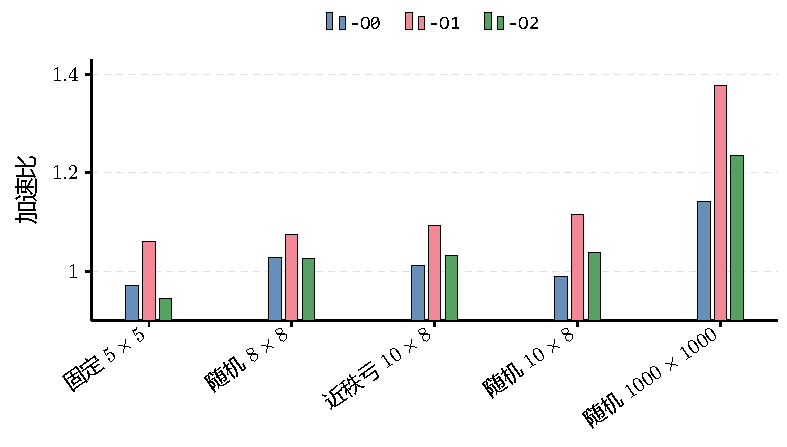
\includegraphics[width=0.6\textwidth]{fig/fig_base_speedup.pdf}
  \caption{不同编译选项与矩阵规模下 SIMD 加速比对比}
  \label{fig:base-speedup}
\end{figure}

表 \ref{tab:base-performance}的结果如下：
\begin{itemize}
  \item 在 \texttt{-O0} 下，上二对角化阶段和 GKH 迭代阶段分别达到 \(1.5950\times\) 和 \(1.0450\times\) 加速，总体加速比为 \(1.1420\times\)。
  \item 在 \texttt{-O1} 下，上二对角化阶段和 GKH 迭代阶段分别达到 \(4.0512\times\) 和 \(1.0578\times\) 加速，总体加速比为 \(1.3764\times\)，是三种编译配置中总体加速最明显的一组。
  \item 在主结果配置 \texttt{-O2} 下，上二对角化阶段和 GKH 迭代阶段分别达到 \(1.8785\times\) 和 \(1.1330\times\) 加速，总体加速比为 \(1.2342\times\)。这说明当前二路 SIMD 在高等级编译优化下仍然能够取得正收益。
\end{itemize}

\subsubsection{基础结果分析}
从表 \ref{tab:base-performance} 可以看出，本次 SIMD 优化对大规模矩阵的收益更明显，但对小规模矩阵收益有限，结果大多在 \(1\times\) 附近。小规模用例中，\texttt{-O0} 下基本持平，\texttt{-O1} 下均有小幅加速，\texttt{-O2} 下除固定值 \(5\times5\) 外也表现为小幅加速。

首先，小规模矩阵本身计算量很小，函数调用、循环控制、向量寄存器初始化和尾部标量处理的固定开销占比较大，因此即使单次向量计算更快，也不足以抵消这些额外成本。其次，本次优化集中在 \texttt{apply\_left\_rows} 和 Householder 相关更新循环，而对于 \(5\times5\)、\(8\times8\)、\(10\times8\) 这样的规模，真正能进入长向量循环的元素数量非常有限，SIMD 的并行度难以充分发挥。

相比之下，在 \(1000\times1000\) 的大规模测试中，Householder 变换和 GKH 迭代都包含大量重复的向量加法、乘法和内积计算，连续内存访问的优势开始体现出来。特别是将原先按列累加的写法改为按行连续访问后，更符合当前矩阵的 row-major 存储方式，降低了访存开销。因此 \texttt{-O0}、\texttt{-O1} 和 \texttt{-O2} 下分别取得 \(1.1420\times\)、\(1.3764\times\) 和 \(1.2342\times\) 的总体加速。

把不同编译优化选项也放在同一条性能比较线上看，可以更清楚地发现：手工 SIMD 与编译器优化并不是简单叠加关系。本文后续选择 \texttt{-O2} 作为主结果配置，是因为它更接近正式性能测试中常用的高优化编译方式。三次平均后，\texttt{-O2} 下原始串行版本总时间为 38588.25 ms，SIMD 版本总时间为 31265.19 ms，总体加速比为 \(1.2342\times\)。其中，上二对角化阶段加速更明显，而 GKH 阶段也取得 \(1.1330\times\) 的加速；因此主配置下的分析重点是说明 SIMD 收益主要来自连续访存的 Householder 相关循环，而 GKH 右列旋转仍是限制进一步提速的主要瓶颈。

\subsection{Profiling 分析}

\subsubsection{Profiling 方法}
在这里进一步使用 \texttt{perf} 对原始版本和 SIMD 版本进行分析。Profiling 包含两类结果：第一类是 \texttt{perf record} 采集的 \texttt{cycles:u} 调用图，用于判断热点函数；第二类是补充的 \texttt{perf stat -r} 统计结果，用于观察 \texttt{cycles}、\texttt{instructions}、cache miss 和 branch miss 等硬件事件。

\begin{algorithm}[H]
\begin{lstlisting}[language=bash]
perf record -g -e cycles:u ./main
perf report --stdio > perf-Ox.txt
perf stat -r 3 -e task-clock,cycles,instructions,branches,branch-misses,cache-references,cache-misses,L1-dcache-loads,L1-dcache-load-misses ./main 2412439
\end{lstlisting}
\caption{Profiling 命令}
\label{alg:profiling-command}
\end{algorithm}

需要说明的是，本次 \texttt{perf} 采样覆盖的是完整测试程序，因此除了核心 SVD 计算外，也包含了 \texttt{reconstruction\_error}、\texttt{orth\_error} 等正确性检查函数的开销。并且补充的 \texttt{perf stat} 是在登录节点终端环境下直接运行得到的，没有通过课程提交脚本进入正式计算节点，因此它的 \texttt{task-clock} 和程序运行时间不能与 \texttt{test.sh} 得到的正式性能数据直接对齐。本文只使用这些 profiling 结果分析同一登录节点环境下的硬件事件相对趋势和热点分布；最终运行时间结论仍以 \texttt{test.sh} 输出为准。

\begin{table}[H]
  \centering
  \small
  \begin{tabular}{ccccc}
    \toprule
    编译选项 & 版本 & 样本数 & \texttt{cycles:u} 事件数 & 相对原始版本 \\
    \midrule
    \texttt{-O0} & 原始版本 & 26K & 673.76G & 1.0000 \\
    \texttt{-O0} & SIMD 版本 & 22K & 579.17G & 0.8596 \\
    \texttt{-O1} & 原始版本 & 7K & 183.36G & 1.0000 \\
    \texttt{-O1} & SIMD 版本 & 6K & 156.33G & 0.8526 \\
    \texttt{-O2} & 原始版本 & 3K & 94.53G & 1.0000 \\
    \texttt{-O2} & SIMD 版本 & 3K & 95.03G & 1.0053 \\
    \bottomrule
  \end{tabular}
  \caption{Profiling 采样结果概要}
  \label{tab:profiling-summary}
\end{table}

\begin{table}[H]
  \centering
  \small
  \resizebox{\textwidth}{!}{
  \begin{tabular}{ccccccc}
    \toprule
    编译选项 & 版本 & \texttt{task-clock}/s & \texttt{cycles}/G & \texttt{instructions}/G & IPC & cache miss 率 \\
    \midrule
    \texttt{-O0} & 原始版本 & 283.80 & 729.29 & 1414.54 & 1.94 & 0.43\% \\
    \texttt{-O0} & SIMD 版本 & 274.07 & 703.57 & 1122.47 & 1.60 & 0.46\% \\
    \texttt{-O1} & 原始版本 & 64.55 & 165.91 & 217.67 & 1.31 & 1.79\% \\
    \texttt{-O1} & SIMD 版本 & 86.76 & 221.54 & 170.69 & 0.77 & 2.80\% \\
    \texttt{-O2} & 原始版本 & 52.33 & 134.11 & 118.95 & 0.89 & 4.69\% \\
    \texttt{-O2} & SIMD 版本 & 50.25 & 128.73 & 97.11 & 0.75 & 5.38\% \\
    \bottomrule
  \end{tabular}}
  \caption{\texttt{perf stat} 硬件事件统计}
  \label{tab:perf-stat-summary}
\end{table}

表 \ref{tab:perf-stat-summary} 可以看到手工 SIMD 改写确实减少了动态指令数：在 \texttt{-O0}、\texttt{-O1} 和 \texttt{-O2} 下，SIMD 版本的 \texttt{instructions} 分别约为原始版本的 79.35\%、78.42\% 和 81.63\%。这说明向量化和按行连续访问改写减少了部分循环中的标量操作数量。

但是，指令数下降并不必然带来同等比例的运行时间下降。以主配置 \texttt{-O2} 为例，SIMD 版本的动态指令数从 118.95G 降至 97.11G，约为原始版本的 81.63\%；如果程序主要受算术指令数量限制，理论上应看到更接近这一比例的运行时间下降。但 \texttt{perf stat} 中总 \texttt{cycles} 只是从 134.11G 降至 128.73G，约为原始版本的 95.99\%，下降幅度明显小于指令数下降幅度。这说明 SIMD 改写减少了需要执行的指令，但每条指令平均消耗的周期变多了。

这一点可以从 IPC 和 cache miss 率看出来。\texttt{-O2} 下原始版本 IPC 为 0.89，而 SIMD 版本为 0.75；同时 cache miss 率从 4.69\% 上升到 5.38\%。IPC 下降说明处理器流水线中有更多周期没有成功退休指令，可能来自数据依赖、访存等待、向量归约的水平求和开销，以及剩余热点中不连续访问造成的停顿。cache miss 率上升则说明当前程序仍有相当一部分时间耗在访存层次上，特别是 GKH 迭代中的右列旋转在 row-major 存储下按列访问，空间局部性较差。也就是说，SIMD 能减少连续向量操作中的算术和循环控制指令，但不能自动消除不连续访存带来的 cache 行利用率问题。

不同优化级别下的现象也支持这一解释。\texttt{-O0} 下 SIMD 版本的指令数和 cycles 都略有下降，因此可以解释其正式测试中的小幅加速；\texttt{-O1} 下虽然指令数减少到原始版本的 78.42\%，但 \texttt{perf stat} 中 cycles 和 task-clock 反而上升，说明该组 profiling 更容易受到运行环境和访存行为影响，不能直接替代正式计时；\texttt{-O2} 下 SIMD 版本的 task-clock 和 cycles 均略低于原始版本，与正式三次平均计时中的总体加速方向一致。由于 \texttt{perf stat} 是在登录节点直接运行得到的，本文最终运行时间结论仍采用 \texttt{test.sh} 三次重复取平均的结果；这里的硬件事件主要用于解释“为什么实际加速低于指令数下降比例”。

\subsubsection{热点函数与瓶颈}

\begin{table}[H]
  \centering
  \small
  \renewcommand{\arraystretch}{1.20}
  \begin{tabularx}{\textwidth}{L{1.20cm}L{1.7cm}L{6cm}Y}
    \toprule
    \textbf{编译选项} & \textbf{版本} & \textbf{主要热点} & \textbf{分析结论} \\
    \midrule
    \texttt{-O0} & 原始版本 & \texttt{gkh\_svd\_from\_bidiagonal} 53.06\%，\newline 其中 \texttt{one\_block\_step} 43.83\% \newline \texttt{apply\_right\_cols} 22.65\%；\newline \texttt{to\_bidiagonal} 12.70\% & 主要热点在 GKH 迭代，右列旋转和矩阵访问开销明显；上二对角化仍有可优化空间。 \\
    \texttt{-O0} & SIMD 版本 & \texttt{gkh\_svd\_from\_bidiagonal} 53.02\%，\newline \texttt{apply\_right\_cols} 25.45\% \newline \texttt{axpy\_simd} 6.87\%，\newline \texttt{dot\_product\_simd} 3.49\% & SIMD 后总 \texttt{cycles} 降低约 14.04\%，但最大热点仍是未被充分向量化的 \texttt{apply\_right\_cols}。 \\
    \addlinespace[0.25em]
    \texttt{-O1} & 原始版本 & \texttt{apply\_right\_cols} 53.18\%，\newline \texttt{to\_bidiagonal} 20.00\% \newline \texttt{cleanup\_bidiagonal} 4.53\% & 编译器优化后热点更集中，GKH 右列旋转成为最主要瓶颈。 \\
    \texttt{-O1} & SIMD 版本 & \texttt{apply\_right\_cols} 61.49\%，\newline \texttt{axpy\_simd} 4.00\% \newline\texttt{apply\_left\_rows} 3.23\%， \newline \texttt{dot\_product\_simd} 2.44\% & 总 \texttt{cycles} 降低约 14.74\%，与 \texttt{-O1} 对照配置中的整体加速现象一致；剩余瓶颈进一步集中到按列访问的右旋转。 \\
    \addlinespace[0.25em]
    \texttt{-O2} & 原始版本 & \texttt{apply\_right\_cols} 47.51\%，\newline \texttt{to\_bidiagonal} 22.52\%，\newline \texttt{cleanup\_bidiagonal} 9.29\% & 原始版本的上二对角化阶段仍占较高比例，因此 SIMD 改写在该阶段有机会取得明显收益。 \\
    \texttt{-O2} & SIMD 版本 & \texttt{apply\_right\_cols} 57.31\%，\newline \texttt{cleanup\_bidiagonal} 10.12\%，\newline \texttt{axpy\_simd} 7.44\%，\newline \texttt{dot\_product\_simd} 5.25\% & 主配置下 \texttt{perf} 事件数与原始版本基本持平，正式三次平均计时中 SIMD 仍取得总体加速；剩余热点主要集中在右列旋转和 GKH 相关更新。 \\
    \bottomrule
  \end{tabularx}
  \renewcommand{\arraystretch}{1.08}
  \caption{Profiling 热点函数}
  \label{tab:profiling}
\end{table}

从热点分布看，SIMD 改写确实降低了部分向量内积和 AXPY 更新的开销：在 \texttt{-O0} 和 \texttt{-O1} 下，SIMD 版本的 \texttt{cycles:u} 事件数分别约为原始版本的 85.96\% 和 85.26\%；在 \texttt{-O2} 下，\texttt{perf stat} 中 SIMD 版本的总 cycles 也略低于原始版本。这与大规模矩阵上三次平均运行时间下降的现象相互印证。

不过，profiling 也说明当前优化并没有触及最主要的剩余热点。\texttt{apply\_right\_cols} 在 \texttt{-O1} SIMD 版本中占到 61.49\%，在 \texttt{-O2} SIMD 版本中占到 57.31\%。该函数对应 GKH 迭代中的右列旋转，在 row-major 矩阵存储下访问列元素时空间局部性较差，因此即使左行旋转和 Householder 更新已经向量化，整体性能仍会继续受到 GKH 阶段限制。

总体上，当前 profiling 可以把性能现象解释为两层：一方面，\texttt{perf stat} 显示手工 SIMD 改写减少了动态指令数和部分内存访问次数；另一方面，\texttt{perf record} 显示热点仍集中在按列访问的 GKH 右旋转操作。也就是说，SIMD 优化确实改善了 Householder 和左行旋转中的一部分连续访问循环，并在三次平均计时中带来了总体加速；但程序的剩余瓶颈仍集中在空间局部性较差、当前尚未充分向量化的右列旋转上。branch miss 数量在各版本之间变化不大，不能作为主要解释；cache miss 率和 IPC 的变化更能说明为什么实际加速比低于纯指令数下降幅度。

\subsection{不同并行度的性能对比}
本节统一以 \texttt{-O2} 作为主结果配置，比较二路、四路和八路 SIMD 展开粒度对性能的影响。需要注意，AArch64 NEON 对 \texttt{double} 的硬件向量宽度仍然是 128 bit，即一个 \texttt{float64x2\_t} 一次处理 2 个元素；这里的二路是最初的 SIMD 改进版，四路和八路则分别指在一个循环体中使用两个或四个 NEON 向量进行手工展开，而不是硬件寄存器本身变宽。因此，四路和八路版本主要通过减少循环控制开销、增加指令级并行机会来影响性能，并不能把单条向量指令的硬件并行宽度从 2 个 \texttt{double} 提高到 4 个或 8 个。

其中二路、四路和八路版本均重复运行 3 次并取平均值，用于观察展开粒度变化带来的趋势。

\begin{table}[H]
  \centering
  \small
  \begin{tabular}{ccccc}
    \toprule
    矩阵规模 & 二路总时间/ms & 四路总时间/ms & 八路总时间/ms & 最优实现 \\
    \midrule
    固定值 $5\times5$ & 0.04993 & 0.04846 & 0.06149 & 四路略快 \\
    随机 $8\times8$ & 0.02627 & 0.02543 & 0.02586 & 四路略快 \\
    近秩亏损 $10\times8$ & 0.02710 & 0.02646 & 0.02678 & 四路略快 \\
    随机 $10\times8$ & 0.02392 & 0.02362 & 0.02928 & 四路略快 \\
    随机 $1000\times1000$ & 31265.19 & 36853.50 & 29376.98 & 八路更优 \\
    \bottomrule
  \end{tabular}
  \caption{不同 SIMD 展开粒度性能对比（\texttt{-O2}，三次平均）}
  \label{tab:simd-width}
\end{table}

从表 \ref{tab:simd-width} 可以看到，小规模样例中二路、四路和八路的差异很小，几种实现的总时间只相差 \(10^{-4}\sim10^{-3}\) ms 量级。对于这些矩阵，循环体本身很短，函数调用、分支判断、收敛控制和计时精度带来的固定开销已经足以掩盖循环展开粒度的影响，因此不能根据小规模样例判断更大的展开因子一定更快。

在随机 \(1000\times1000\) 样例上，二路版本三次平均总时间为 31265.19 ms，其中上二对角化阶段 4244.66 ms，GKH 迭代阶段 27020.53 ms；四路版本总时间为 36853.50 ms，其中上二对角化阶段 4571.87 ms，GKH 迭代阶段 32281.63 ms；八路版本总时间为 29376.98 ms，其中上二对角化阶段 3211.25 ms，GKH 迭代阶段 26165.73 ms。相对于二路版本，八路版本总加速比为 \(1.0643\times\)，总时间降低约 6.04\%；其中上二对角化阶段加速约 \(1.3218\times\)，GKH 阶段加速约 \(1.0327\times\)。四路版本相对于二路版本总时间反而增加约 17.87\%，说明适度展开并不必然带来收益。

这一现象说明，手工展开粒度与实际性能之间不是单调关系。二路、四路和八路都建立在 \texttt{float64x2\_t} 之上，硬件层面每条 NEON 指令仍然只处理 2 个 \texttt{double}。八路版本在本次三次平均中表现最好，主要是因为它在大规模矩阵上进一步减少了循环控制开销，并让上二对角化中的连续向量操作获得更高吞吐；但四路版本在 GKH 阶段耗时较高，说明展开后的寄存器占用、指令调度和访存行为也可能抵消一部分收益。因此，更大的展开因子并不等价于更高的硬件 SIMD 并行度。

\begin{figure}[H]
  \centering
  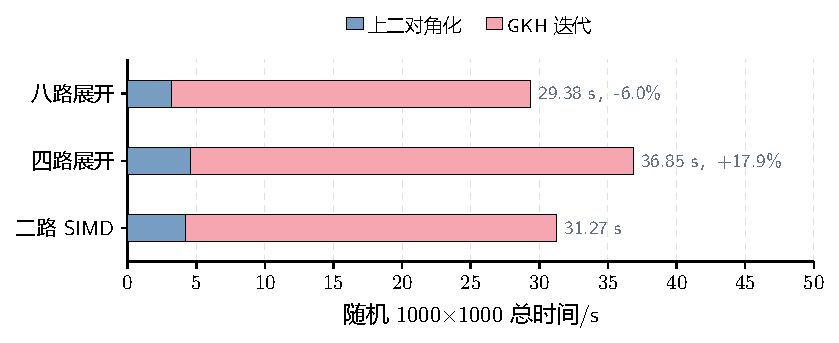
\includegraphics[width=0.66\textwidth]{fig/fig_simd_width_1000_stacked.pdf}
  \caption{随机 \(1000\times1000\) 样例上不同 SIMD 展开粒度的分阶段耗时对比}
  \label{fig:simd-width}
\end{figure}

\subsection{不同编译优化选项对性能的影响}
本节单独比较不同编译优化选项对原始版本和 SIMD 版本性能的影响。为了避免小规模矩阵计时噪声干扰，表 \ref{tab:compile-options} 只列出随机 \(1000\times1000\) 用例三次平均后的正式测试结果；\texttt{perf stat} 的硬件事件作为辅助解释，不直接替代这里的运行时间。

\begin{table}[H]
  \centering
  \small
  \begin{tabular}{ccccc}
    \toprule
    编译选项 & 原始版本时间/ms & SIMD 版本时间/ms & 加速比 & 主要现象 \\
    \midrule
    \texttt{-O0} & 158294.47 & 138616.20 & 1.1420 & SIMD 有效，但编译器自身优化不足 \\
    \texttt{-O1} & 47072.37 & 34199.00 & 1.3764 & 对照配置中加速最明显 \\
    \texttt{-O2} & 38588.25 & 31265.19 & 1.2342 & 主配置下取得总体加速 \\
    \bottomrule
  \end{tabular}
  \caption{不同编译优化选项性能对比}
  \label{tab:compile-options}
\end{table}

从原始版本看，编译优化本身的收益非常明显：从 \texttt{-O0} 到 \texttt{-O1}，总时间由 158294.47 ms 降到 47072.37 ms；进一步到 \texttt{-O2} 后降到 38588.25 ms。这说明原始串行代码中存在大量可由编译器处理的循环优化、内联和常量传播机会。对应的 \texttt{perf stat} 也显示，原始版本的动态指令数从 \texttt{-O0} 的 1414.54G 降到 \texttt{-O2} 的 118.95G，\texttt{cycles} 从 729.29G 降到 134.11G，编译器优化对标量代码非常关键。

对 SIMD 版本而言，性能随编译优化级别变化并不是单调的。\texttt{-O0} 下 SIMD 通过手工向量化取得 \(1.1420\times\) 加速，说明即使编译器不做较强优化，NEON intrinsic 和按行连续访问改写也能减少部分计算开销；\texttt{-O1} 下加速比进一步提升到 \(1.3764\times\)，说明基本循环优化和手工 SIMD 能够形成较好的配合。\texttt{-O2} 下加速比为 \(1.2342\times\)，仍然保持正收益。本文选择 \texttt{-O2} 作为主结果配置，因为它更符合最终提交和高性能程序通常使用的优化等级，也更适合检验手工 SIMD 在强编译器优化之后是否仍有稳定收益。

\texttt{-O2} 的结果说明，手工 SIMD 与高等级编译优化并不是简单叠加关系。三次平均结果中，SIMD 版本的上二对角化阶段从 7973.45 ms 降至 4244.66 ms，加速约 \(1.8785\times\)；GKH 迭代阶段从 30614.80 ms 降至 27020.53 ms，加速约 \(1.1330\times\)。结合 \texttt{perf stat} 可见，\texttt{-O2} 下 SIMD 版本的动态指令数和总 cycles 均低于原始版本，但它的 IPC 更低、cache miss 率更高，并且 \texttt{perf record} 中 \texttt{apply\_right\_cols} 仍占最大热点。这说明 SIMD 指令减少了部分计算量并带来了总体加速，但 GKH 右列旋转的访存模式仍然限制了进一步提速。

\section{进阶要求}

\subsection{进阶要求概述}
根据题目要求，进阶部分主要围绕更深入的对比实验和进一步优化展开。本文将进阶要求组织为三个部分：手工编写的 SIMD 程序与编译器自动向量化版本的对比实验及性能分析；不同平台 SIMD 并行化的对比实验及性能分析；其他算法优化策略。

\subsection{手工编写的 SIMD 程序与编译器自动向量化版本的对比}
本部分用于比较手工编写 NEON intrinsic 的版本与仅依赖编译器自动向量化的版本在正确性、运行时间和加速比方面的差异。本节额外设置了一个禁止自动向量化的基线版本。三个版本均使用相同随机种子 \texttt{2412439} 和相同测试集，并直接运行 \texttt{./main 2412439} 收集输出。

\begin{table}[H]
  \centering
  \small
  \renewcommand{\arraystretch}{1.16}
  \begin{tabularx}{\textwidth}{L{2.1cm}L{3.0cm}R{2.0cm}R{1.6cm}R{1.9cm}Y}
    \toprule
    实现方式 & 编译选项 & 上二对角化/ms & GKH/ms & 总时间/ms & 备注 \\
    \midrule
    禁用向量化基线 & \begin{tabular}[t]{@{}l@{}}\texttt{-O2}\\\texttt{-fno-tree-vectorize}\end{tabular} & 9381.49 & 47011.40 & 56392.89 & 标量源码，显式关闭编译器向量化 \\
    自动向量化 & \begin{tabular}[t]{@{}l@{}}\texttt{-O2}\\\texttt{-ftree-vectorize}\end{tabular} & 7973.45 & 30614.80 & 38588.25 & 标量源码，允许编译器自动生成 SIMD \\
    手工 SIMD（二路） & \begin{tabular}[t]{@{}l@{}}\texttt{-O2}\\\texttt{-ftree-vectorize}\end{tabular} & 4244.66 & 27020.53 & 31265.19 & NEON intrinsic 手工改写核心循环 \\
    \bottomrule
  \end{tabularx}
  \renewcommand{\arraystretch}{1.08}
  \caption{手工 SIMD 与编译器自动向量化版本性能对比（随机 \(1000\times1000\)，\texttt{-O2}）}
  \label{tab:auto-vs-manual}
\end{table}

表 \ref{tab:auto-vs-manual} 中的加速比以“禁用向量化基线”为参照。自动向量化版本总时间由 56392.89 ms 降至 38588.25 ms，加速比约为 \(1.4614\times\)，总时间降低约 31.57\%。分阶段看，上二对角化阶段加速约 \(1.1766\times\)，GKH 阶段加速约 \(1.5356\times\)。这说明在原始标量源码上，编译器的 loop vectorization 和相关循环优化确实能够识别并优化一部分连续访存和简单线性代数循环。

手工 SIMD 二路版本相对于禁用向量化基线也有提升，总加速比约为 \(1.8037\times\)，总时间降低约 44.56\%。其中上二对角化阶段从 9381.49 ms 降至 4244.66 ms，加速约 \(2.2102\times\)，说明 \texttt{dot\_product\_simd}、\texttt{self\_dot\_simd} 和 \texttt{axpy\_simd} 等手工 NEON 改写对 Householder 阶段是有效的；GKH 阶段从 47011.40 ms 降至 27020.53 ms，加速约 \(1.7398\times\)，也取得了明显收益。

进一步比较自动向量化和手工 SIMD 二路版本，自动向量化总时间为 38588.25 ms，手工 SIMD 二路总时间为 31265.19 ms，手工 SIMD 二路比自动向量化快约 18.98\%。这说明当前手工 SIMD 不只是替代编译器自动向量化，而是在 Householder 相关连续向量操作上进一步扩大了收益；同时，\texttt{apply\_right\_cols} 这类按列访问的 GKH 热点仍在 profiling 中占比较高，若要继续提升速度，仍需要围绕右列旋转、访存布局和寄存器调度做更深入优化。

为了进一步解释自动向量化和手工 SIMD 的差异，本文额外收集了 \texttt{perf stat}、\texttt{perf record} 和 GCC 向量化报告。这里的手工 SIMD 辅助实验使用 \texttt{-O2 -fno-tree-vectorize} 编译，目的是隔离手写 NEON intrinsic 本身的作用；而表 \ref{tab:auto-vs-manual} 中最终采用的手工 SIMD 主结果仍使用 \texttt{-O2}，保留编译器对其他标量循环的常规优化。

\begin{table}[H]
  \centering
  \small
  \renewcommand{\arraystretch}{1.16}
  \begin{tabularx}{\textwidth}{L{2.75cm}L{3.05cm}R{1.85cm}R{1.75cm}R{1.8cm}C{2.1cm}}
    \toprule
    版本 & 编译选项 & 上二对角化/ms & GKH/ms & 总时间/ms & 相对禁用向量化加速比 \\
    \midrule
    禁用向量化基线 & \begin{tabular}[t]{@{}l@{}}\texttt{-O2}\\\texttt{-fno-tree-vectorize}\end{tabular} & 10976.83 & 63410.30 & 74387.13 & 1.0000 \\
    自动向量化 & \begin{tabular}[t]{@{}l@{}}\texttt{-O2}\\\texttt{-ftree-vectorize}\end{tabular} & 6503.69 & 39265.77 & 45769.46 & 1.6253 \\
    手工 SIMD（关闭自动向量化） & \begin{tabular}[t]{@{}l@{}}\texttt{-O2}\\\texttt{-fno-tree-vectorize}\end{tabular} & 4692.13 & 43781.33 & 48473.46 & 1.5346 \\
    \bottomrule
  \end{tabularx}
  \renewcommand{\arraystretch}{1.08}
  \caption{自动向量化与手工 SIMD 的登录节点辅助计时（随机 \(1000\times1000\)，三次平均）}
  \label{tab:auto-profiling-time}
\end{table}

\begin{table}[H]
  \centering
  \scriptsize
  \resizebox{\textwidth}{!}{
  \begin{tabular}{p{3.0cm}ccccc}
    \toprule
    版本 & \texttt{task-clock}/s & \texttt{cycles}/G & \texttt{instructions}/G & IPC & L1 dcache miss 率 \\
    \midrule
    禁用向量化基线 & 79.96 & 204.20 & 118.95 & 0.58 & 5.67\% \\
    自动向量化 & 48.99 & 124.14 & 87.65 & 0.71 & 6.81\% \\
    手工 SIMD（关闭自动向量化） & 54.57 & 139.09 & 97.11 & 0.70 & 5.53\% \\
    \bottomrule
  \end{tabular}}
  \caption{自动向量化与手工 SIMD 的登录节点 \texttt{perf stat} 结果}
  \label{tab:auto-profiling-stat}
\end{table}

从 profiling 看，自动向量化版本相对于禁用向量化基线，将 \texttt{cycles} 降至约 60.79\%，将动态指令数降至约 73.69\%；手工 SIMD 在关闭编译器自动向量化后，\texttt{cycles} 降至约 68.11\%，动态指令数降至约 81.64\%。这说明两种方式都减少了实际执行的指令和周期数。自动向量化在该辅助实验中的总时间略优于“关闭自动向量化的手工 SIMD”，并不否定主结果中手工 SIMD 的收益，而是说明完整程序还依赖编译器对未手写 SIMD 的剩余循环进行优化。最终提交版本采用的是手工 NEON intrinsic 与 \texttt{-O2} 编译优化共同作用的结果。

\begin{table}[H]
  \centering
  \small
  \renewcommand{\arraystretch}{1.20}
  \begin{tabularx}{\textwidth}{L{3.55cm}L{3.95cm}Y}
    \toprule
    \textbf{报告位置} & \textbf{对应代码含义} & \textbf{分析} \\
    \midrule
    \texttt{gkh.cpp:26} & \texttt{apply\_left\_rows} 的逐列两行旋转 & 该循环按行连续访问，两行元素可以顺序加载，因此 GCC 能使用 16 Byte 向量进行自动向量化。 \\
    \begin{tabular}[t]{@{}l@{}}\texttt{bidiagonalization.cpp}\\\texttt{:96/106}\end{tabular} & 左 Householder 作用到 \(B\) 和累积 \(U\) 的内层更新循环 & 更新形式接近 AXPY，内层按连续列访问，适合自动向量化，但编译器仍需要做 alias 版本化检查。 \\
    \begin{tabular}[t]{@{}l@{}}\texttt{bidiagonalization.cpp}\\\texttt{:159/169}\end{tabular} & 右 Householder 作用到 \(B\) 和累积 \(V\) 的内层更新循环 & 内层同样是连续行片段上的线性更新，因此可以被自动向量化。 \\
    \texttt{matrix.h:42} 等 & 矩阵初始化、复制或 STL 容器内部循环 & 属于辅助数据搬运，能减少部分开销，但不是最终性能瓶颈。 \\
    未出现在主要向量化列表中的热点 & \texttt{apply\_right\_cols} & 该函数在 row-major 存储下按列跨步访问，仍在 \texttt{perf record} 中占据主要热点，因此是自动向量化和当前手工 SIMD 都未充分解决的瓶颈。 \\
    \bottomrule
  \end{tabularx}
  \renewcommand{\arraystretch}{1.08}
  \caption{GCC 自动向量化报告摘要}
  \label{tab:vec-report}
\end{table}

表 \ref{tab:vec-report} 说明，GCC 自动向量化主要覆盖了两类循环：一类是 \texttt{apply\_left\_rows} 这种按行连续访问的旋转更新，另一类是 Householder 阶段中形如内积或 AXPY 的连续线性更新。它们的共同特点是内层循环访问地址连续、循环边界清晰、运算形式简单，编译器较容易判断每次迭代之间不存在复杂依赖，因此能够生成 16 Byte 宽度的向量化代码。对于 \texttt{bidiagonalization.cpp} 中的若干循环，报告中还出现了 alias 版本化检查，说明 GCC 会在运行时区分指针是否可能重叠：若判断不重叠，就进入向量化路径；否则回退到保守的标量路径。

但这张表也解释了自动向量化的局限。报告中能看到的主要是“局部规则循环”被向量化，而完整程序的最大热点 \texttt{apply\_right\_cols} 并未出现在主要向量化列表中。该函数在 row-major 存储下按列跨步访问，同一列相邻元素在内存中并不连续，cache line 利用率低，也不适合直接映射为连续 SIMD load/store。因此，自动向量化虽然能减少一部分动态指令数并提升局部循环吞吐，但无法从根本上解决 GKH 右列旋转的访存瓶颈。这也是前文中自动向量化取得总体加速、但加速比仍受限的重要原因。

\texttt{perf record} 的热点分布进一步印证了这一点：禁用向量化基线中 \texttt{apply\_right\_cols} 约占 80.70\%，自动向量化版本中仍约占 82.78\%；手工 SIMD 辅助版本中该热点下降到约 59.59\%，同时 \texttt{axpy\_simd} 和 \texttt{dot\_product\_simd} 分别占 6.72\% 和 4.39\%。这说明手工 SIMD 把一部分 Householder 连续向量操作显式改写成 NEON 指令后，热点结构发生了变化；但只要 GKH 右列旋转仍按列跨步访问，完整程序的上限就仍然受到该函数限制。

\subsection{不同平台 SIMD 并行化的对比实验及性能分析}
本部分用于比较不同平台上的 SIMD 并行化效果。需要注意的是，不同平台之间 CPU 主频、微架构、缓存层次、内存带宽和编译器实现均不相同，因此不能简单用绝对运行时间判断某个平台的 SIMD 指令集“更强”。本文采用平台内归一化方式：分别在每个平台上测试禁止自动向量化的标量基线和手工 SIMD 版本，再比较平台内加速比。

为了保证比较口径清楚，两个平台的标量基线均使用 \texttt{-O2 -fno-tree-vectorize}，即保留编译器常规优化但禁止自动向量化；手工 SIMD 版本也使用 \texttt{-O2 -fno-tree-vectorize}，区别仅在于源码中显式写入 SIMD intrinsic。ARM 平台采用单独收集的 AArch64 NEON 二路手工 SIMD 结果；x86 平台在本机 Windows 11 环境下加入 AVX 分支，并额外使用 \texttt{-mavx} 打开 AVX 指令。

\begin{algorithm}[H]
\begin{lstlisting}[language=bash]
# ARM 标量基线
g++ main.cpp gkh.cpp bidiagonalization.cpp -o main \
  -O2 -fno-tree-vectorize -fopenmp -lpthread -std=c++17

# ARM 手工 NEON
g++ main.cpp gkh.cpp bidiagonalization.cpp -o main \
  -O2 -fno-tree-vectorize -fopenmp -lpthread -std=c++17

# x86 标量基线
g++ main.cpp gkh.cpp bidiagonalization.cpp -o main_x86_scalar.exe \
  -O2 -fno-tree-vectorize -fopenmp -lpthread -std=c++17

# x86 手工 AVX
g++ main.cpp gkh.cpp bidiagonalization.cpp -o main_x86_avx.exe \
  -O2 -mavx -fno-tree-vectorize -fopenmp -lpthread -std=c++17
\end{lstlisting}
\caption{不同平台对比实验的编译命令}
\label{alg:platform-compile}
\end{algorithm}

本机 x86 AVX 版本在 \texttt{bidiagonalization.cpp} 的 \texttt{dot\_product\_simd}、\texttt{self\_dot\_simd}、\texttt{axpy\_simd} 以及 \texttt{gkh.cpp} 的 \texttt{apply\_left\_rows} 中加入了 \texttt{\_\_m256d} 分支。AVX 的 256 bit 向量寄存器一次可处理 4 个 \texttt{double}，而 AArch64 NEON 的 128 bit 向量寄存器一次处理 2 个 \texttt{double}。

\begin{table}[H]
  \centering
  \footnotesize
  \renewcommand{\arraystretch}{1.18}
  \begin{tabularx}{\textwidth}{L{2.15cm}L{3.05cm}L{3.05cm}Y}
    \toprule
    \textbf{对比项} & \textbf{ARM AArch64 NEON} & \textbf{x86\_64 AVX} & \textbf{对本实验的影响} \\
    \midrule
    实际测试平台 & HiSilicon Kunpeng-920\newline GCC 10.3.1 & Intel Core i7-13650HX\newline GCC 15.1.0 & 两个平台不仅 SIMD 指令集不同，CPU 微架构、编译器版本和运行环境也不同，因此跨平台绝对时间不能直接作为指令集优劣判断。 \\
    向量寄存器宽度 & 128 bit，双精度下一条向量指令处理 2 个元素 & 256 bit，双精度下一条向量指令处理 4 个元素 & AVX 在连续内存的内积、平方和、AXPY 中有更高的理论数据并行度；但只有热点循环能够连续访存时，这个优势才能体现出来。 \\
    向量寄存器数量 & AArch64 提供 32 个 128 bit 向量寄存器 & x86\_64 AVX 通常提供 16 个 256 bit YMM 寄存器 & x86 单条指令更宽，但可同时保存的独立向量数量未必更多；在展开和归约循环中，寄存器压力、临时变量和调度开销可能抵消部分宽向量收益。 \\
    访存粒度与 cache 行利用 & NEON 每次向量 load/store 覆盖 16 Byte & AVX 每次向量 load/store 覆盖 32 Byte & 对按行连续访问，AVX 可以用更少指令搬运同样数据；对 \texttt{apply\_right\_cols} 这类按列跨步访问，二者都难以充分利用 cache line，宽向量并不能直接解决空间局部性问题。 \\
    当前代码覆盖范围 & 手工 NEON 覆盖 Householder 辅助函数和左行旋转 & 手工 AVX 覆盖对应的连续向量函数和左行旋转 & 两个平台的 SIMD 都没有从根本上改变 GKH 右列旋转的访存模式，因此整体加速主要取决于可向量化部分在总时间中的占比。 \\
    基线性能 & ARM 服务器的标量基线较慢 & 本机 x86 标量基线绝对时间更短 & 绝对时间同时受主频、缓存层次、乱序执行能力、编译器和运行环境影响，因此跨平台不能直接比较总时间，只能比较平台内加速比和阶段趋势。 \\
    \bottomrule
  \end{tabularx}
  \renewcommand{\arraystretch}{1.08}
  \caption{ARM NEON 与 x86 AVX 在本实验中的架构差异}
  \label{tab:platform-arch}
\end{table}

\begin{table}[H]
  \centering
  \small
  \renewcommand{\arraystretch}{1.22}
  \begin{tabularx}{\textwidth}{L{2.0cm}L{2.05cm}R{2.0cm}R{2.0cm}C{1.6cm}Y}
    \toprule
    \textbf{平台} & \textbf{指令集} & \textbf{标量时间/ms} & \textbf{SIMD 时间/ms} & \textbf{平台内加速比} & \textbf{备注} \\
    \midrule
    ARM Linux & NEON 128 bit & 56392.89 & 48354.50 & 1.1662 &
    \begin{tabular}[t]{@{}l@{}}\texttt{-O2}\\\texttt{-fno-tree-vectorize}\\手工 NEON\end{tabular} \\
    Win11 x86\_64 & AVX 256 bit & 12977.07 & 12000.36 & 1.0814 &
    \begin{tabular}[t]{@{}l@{}}\texttt{-O2 -mavx}\\\texttt{-fno-tree-vectorize}\\手工 AVX\end{tabular} \\
    \bottomrule
  \end{tabularx}
  \renewcommand{\arraystretch}{1.08}
  \caption{不同平台 SIMD 并行化性能对比（随机 \(1000\times1000\)）}
  \label{tab:platform-compare}
\end{table}

从表 \ref{tab:platform-compare} 可以看到，x86 平台的绝对运行时间明显短于 ARM 平台，但这不能直接解释为“AVX 一定优于 NEON”。两个平台的 CPU 主频、缓存层次、内存系统、乱序执行能力和编译器实现均不同，绝对时间混合了大量非 SIMD 因素。因此本文采用平台内归一化方式：ARM NEON 相对于 ARM 标量基线的加速比约为 \(1.1662\times\)，x86 AVX 相对于 x86 标量基线的加速比约为 \(1.0814\times\)。这个结果反而说明，向量寄存器更宽并不必然带来更高的完整程序加速比。

进一步拆分阶段看，x86 AVX 在上二对角化阶段从 1933.97 ms 降至 1104.86 ms，加速约 \(1.7504\times\)；但 GKH 阶段仅从 11043.10 ms 降至 10895.50 ms，加速约 \(1.0135\times\)。ARM NEON 也呈现类似趋势：上二对角化阶段加速约 \(2.1671\times\)，GKH 阶段加速约 \(1.0678\times\)。结合表 \ref{tab:platform-arch} 可以解释这一现象：Householder 上二对角化中的 \texttt{dot\_product\_simd}、\texttt{self\_dot\_simd} 和 \texttt{axpy\_simd} 主要访问连续数组，能够较好地转化为向量 load、向量乘加和向量 store；而 GKH 阶段的主要瓶颈 \texttt{apply\_right\_cols} 在 row-major 存储下按列跨步访问，cache line 中被真正使用的数据比例较低，硬件预取和连续向量加载都难以充分发挥作用。

因此，AVX 的 256 bit 宽度虽然使单条指令的理论双精度并行度达到 NEON 的两倍，但这种优势只作用在“数据连续、循环结构简单、依赖关系清晰”的局部循环中。对于完整 SVD 程序，剩余时间主要集中在 GKH 迭代和右列旋转；这部分更受访存局部性、cache miss、循环控制和收敛过程影响，而不是单纯受向量宽度影响。换言之，x86 平台中 AVX 对上二对角化阶段的局部收益很明显，但由于 GKH 阶段占总时间比例较高，整体加速比被稀释；ARM 平台同样如此，只是其标量基线和编译器生成代码的特征不同，使平台内加速比表现略有差异。

这也说明跨平台 SIMD 对比不能只看“NEON 128 bit、AVX 256 bit”这一条指标。更合理的结论是：当前程序的可向量化收益主要由算法热点和数据布局决定，平台 SIMD 宽度只是其中一个因素。若后续希望让 AVX 或 NEON 的架构优势进一步转化为整体性能提升，需要优先处理 \texttt{apply\_right\_cols} 的跨步访存问题，例如改变矩阵布局、增加转置副本，或把右列旋转改写为更连续的批量更新；否则，即使换用更宽的向量指令集，完整程序加速仍会受 GKH 阶段限制。

\subsection{其他算法优化策略：分块 Householder 变换}
除直接改变 SIMD 展开粒度外，本次还尝试了一个独立的分块 Householder 。该版本仍按原始顺序对 \(B\) 执行左右 Householder 消元，以保证双对角化过程稳定；不同之处在于，一个 block 内生成的左、右 Householder 向量会分别暂存起来，并在 block 结束时用 compact WY 形式合并：
\[
  H_0H_1\cdots H_{b-1}=I-YTY^T.
\]
随后再将合并后的反射变换批量作用到 \(U\) 和 \(V\) 上。这样做的目标是减少正交矩阵累积阶段中大量零散的小更新，并让内积和 AXPY 更新继续复用前文的 NEON SIMD 辅助函数。为了判断该算法优化本身是否带来额外收益，本节同时列出原始 \texttt{-O2} 版本、本文默认的二路 SIMD \texttt{-O2} 版本和分块 Householder + SIMD 版本进行比较。

\begin{algorithm}[H]
\begin{lstlisting}[language=C++]
B = A, U = I_m, V = I_n
for block_begin = 0; block_begin < n; block_begin += block_size:
    block_end = min(n, block_begin + block_size)
    left_block = empty, right_block = empty

    for k = block_begin; k < block_end; ++k:
        // 左 Householder: 消去 B(k:m, k) 的对角线以下元素
        (vL, betaL) = householder(B(k:m, k))
        if betaL != 0:
            left_block.push(start=k, v=vL, beta=betaL)
            // B 仍立即更新，内积和 AXPY 使用二路 NEON SIMD
            w = betaL * transpose(vL) * B(k:m, k:n)
            B(k:m, k:n) = B(k:m, k:n) - vL * w

        // 右 Householder: 消去 B(k, k+2:n) 的元素
        if k + 1 < n:
            (vR, betaR) = householder(B(k, k+1:n))
            if betaR != 0:
                right_block.push(start=k+1, v=vR, beta=betaR)
                z = B(k:m, k+1:n) * vR
                B(k:m, k+1:n) = B(k:m, k+1:n) - betaR * z * transpose(vR)

    // block 结束后再批量累计正交矩阵
    U = U * compactWY(left_block)
    V = V * compactWY(right_block)
return B, U, V
\end{lstlisting}
\caption{分块 Householder 原型伪代码}
\label{alg:block-householder}
\end{algorithm}

\begin{table}[H]
  \centering
  \small
  \resizebox{\textwidth}{!}{
  \begin{tabular}{cccccc}
    \toprule
    实现版本 & 上二对角化/ms & GKH/ms & 总时间/ms & 相对原始加速比 & 相对二路 SIMD 加速比 \\
    \midrule
    原始版本（\texttt{-O2}） & 7973.45 & 30614.80 & 38588.25 & 1.0000 & 0.8102 \\
    二路 SIMD（\texttt{-O2}） & 4244.66 & 27020.53 & 31265.19 & 1.2342 & 1.0000 \\
    分块 Householder + SIMD（\texttt{-O2}） & 2812.02 & 30286.27 & 33098.29 & 1.1659 & 0.9446 \\
    \bottomrule
  \end{tabular}}
  \caption{分块 Householder 优化性能对比（随机 \(1000\times1000\)，\texttt{-O2}，三次平均）}
  \label{tab:block-householder}
\end{table}

\begin{figure}[H]
  \centering
  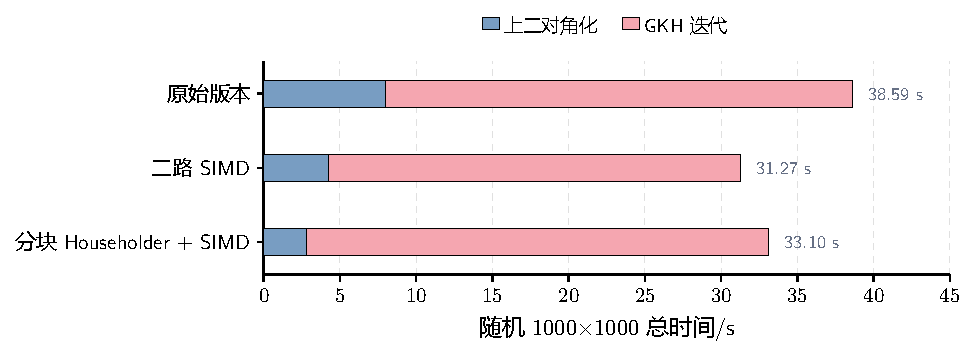
\includegraphics[width=0.90\textwidth]{fig/fig_block_householder_stacked.pdf}
  \caption{随机 \(1000\times1000\) 样例上分块 Householder 与原始、二路 SIMD 的分阶段耗时对比}
  \label{fig:block-householder}
\end{figure}

从表 \ref{tab:block-householder} 和图 \ref{fig:block-householder} 可以看到，分块 Householder 对上二对角化阶段非常有效：相对于原始 \texttt{-O2} 版本，上二对角化从 7973.45 ms 降至 2812.02 ms，加速约 \(2.8355\times\)；相对于二路 SIMD \texttt{-O2} 版本，也从 4244.66 ms 降至 2812.02 ms，仍有约 \(1.5095\times\) 的阶段加速。这说明将一个 block 内的 Householder 变换合并后再更新 \(U\) 和 \(V\)，确实能减少正交矩阵累积过程中的重复访存和更新开销。

不过，分块版本的 GKH 阶段为 30286.27 ms，相对于原始 \texttt{-O2} 版本的 30614.80 ms 仅有 \(1.0108\times\) 的小幅提升；而相对于二路 SIMD \texttt{-O2} 版本的 27020.53 ms，则下降到 \(0.8922\times\)。因此在总时间上，分块版本相对于原始 \texttt{-O2} 版本仍达到 \(1.1659\times\) 加速，但相对于二路 SIMD \texttt{-O2} 版本只有 \(0.9446\times\)，即总时间慢约 5.86\%。这说明当前分块原型的收益主要集中在上二对角化阶段；若要把它转化为更强的整体加速，还需要继续优化 GKH 阶段，或者实现更完整的尾随子矩阵块更新，使分块策略不仅减少 \(U/V\) 累积开销，也能降低核心矩阵更新的访存成本。


\section{总结}
本次实验围绕 SVD 分解中的 SIMD 并行化实现、性能测试和进一步优化展开，主要结论如下：
\begin{enumerate}
  \item \textbf{SIMD 核心实现。} 在 \texttt{gkh.cpp} 中完成了基于 NEON 的两行旋转向量化，并在 Householder 上二对角化部分完成了内积、平方和和行更新的 SIMD 改写；同时通过尾部标量循环保证非整数倍向量宽度规模下的正确处理。
  \item \textbf{正确性验证。} 通过 \texttt{origin} 与 \texttt{version1} 的对比，验证了所有测试用例均能正确收敛；虽然 SIMD 改变了部分浮点运算顺序，但重构误差仍保持在 \(10^{-13}\) 数量级，说明向量化没有破坏 SVD 分解的数值稳定性。
  \item \textbf{SIMD 加速成果。} 在随机 \(1000\times1000\) 大规模测试中，手工 SIMD 取得了明确的总体加速：\texttt{-O0}、\texttt{-O1} 和主结果配置 \texttt{-O2} 下的总体加速比分别为 \(1.1420\times\)、\(1.3764\times\) 和 \(1.2342\times\)。其中，\texttt{-O2} 下总时间由 38588.25 ms 降至 31265.19 ms；上二对角化阶段由 7973.45 ms 降至 4244.66 ms，阶段加速约 \(1.8785\times\)，是 SIMD 收益最集中的部分。
  \item \textbf{相对自动向量化的收益。} 以禁用自动向量化的 \texttt{-O2} 标量版本为基线，手工 SIMD 二路版本总加速比达到 \(1.8037\times\)，总时间降低约 44.56\%；同时相比编译器自动向量化版本仍快约 18.98\%。这说明本次手写 NEON intrinsic 不只是依赖编译器优化，而是在 Householder 连续向量操作上额外扩大了加速效果。
  \item \textbf{展开粒度实验。} 二路、四路和八路展开并不呈现简单的单调关系。小规模样例中展开粒度差异很小；在随机 \(1000\times1000\) 样例上，八路展开版本总时间为 29376.98 ms，相对原始 \texttt{-O2} 版本达到 \(1.3136\times\) 加速，相对二路 SIMD 版本也有 \(1.0643\times\) 的额外提升，说明适当增加循环展开能够继续减少控制开销并提升连续向量循环吞吐。
  \item \textbf{分块 Householder 原型。} 分块 Householder + SIMD 版本将上二对角化阶段进一步降至 2812.02 ms，相对原始 \texttt{-O2} 版本阶段加速约 \(2.8355\times\)，相对二路 SIMD 也有约 \(1.5095\times\) 的阶段加速。
  \item \textbf{瓶颈与后续方向。} 从阶段分析和 \texttt{perf} 热点看，上二对角化中的连续内积、平方和和 AXPY 更新最容易受益于 SIMD，而 GKH 迭代中的右列旋转 \texttt{apply\_right\_cols} 仍受 row-major 存储下跨步访存限制，是进一步提升整体性能的主要瓶颈。后续可围绕矩阵布局调整、转置副本、右列旋转批量更新和更完整的块算法继续优化。
\end{enumerate}

\end{document}
